\documentclass[compress, aspectratio=54]{beamer}
%\documentclass[notes=show]{beamer}
%\documentclass[xcolor=dvipsnames]{beamer}
\usepackage[export]{adjustbox}
\usepackage{sidecap}
\usepackage{subfig}
\usepackage{amssymb}
\usepackage{latexsym}
\usepackage{amsfonts}
\usepackage{amsmath}
\usepackage[absolute,overlay]{textpos}
\usepackage[english]{babel}
\usepackage[latin1]{inputenc}
\usepackage{subfig}
\usepackage{pythontex} 
\usepackage{listings}

%\usepackage{times}
\usepackage[T1]{fontenc}
\usepackage{tabularx}
\newcolumntype{Y}{>{\small\raggedright\arraybackslash}X}
\usepackage{graphicx}
\usepackage{bigstrut}
\usepackage{bbm}
\usepackage{mathrsfs}
\usepackage{epsfig}
\usepackage{array}
%\usepackage{natbib}
\usepackage{hyperref}
\usepackage{caption}
\usepackage{comment}

\mode<presentation> {
%\usetheme[left,width=1.7cm]{Berkeley}
%\usetheme{default}
\usetheme{Boadilla}
  \usecolortheme[RGB={103,102,204}]{structure}
%\usecolortheme{dove}
  \useoutertheme{infolines}
  \setbeamercovered{transparent}
 }

%\usepackage[utf8]{inputenc}

% Default fixed font does not support bold face
\DeclareFixedFont{\ttb}{T1}{txtt}{bx}{n}{12} % for bold
\DeclareFixedFont{\ttm}{T1}{txtt}{m}{n}{12}  % for normal

% Custom colors
\usepackage{color}
\definecolor{deepblue}{rgb}{0,0,0.5}
\definecolor{deepred}{rgb}{0.6,0,0}
\definecolor{deepgreen}{rgb}{0,0.5,0}

\usepackage{listings}

% Python style for highlighting
\newcommand\pythonstyle{\lstset{
language=Python,
basicstyle=\ttm,
otherkeywords={self},             % Add keywords here
keywordstyle=\ttb\color{deepblue},
emph={MyClass,__init__},          % Custom highlighting
emphstyle=\ttb\color{deepred},    % Custom highlighting style
stringstyle=\color{deepgreen},
frame=tb,                         % Any extra options here
showstringspaces=false            % 
}}


% Python environment
\lstnewenvironment{python}[1][]
{
\pythonstyle
\lstset{#1}
}
{}

% Python for external files
\newcommand\pythonexternal[2][]{{
\pythonstyle
\lstinputlisting[#1]{#2}}}

% Python for inline
\newcommand\pythoninline[1]{{\pythonstyle\lstinline!#1!}}
%\renewcommand{\familydefault}{cmss}
%\renewcommand{\mathrm}{\mathsf}
%\renewcommand{\textrm}{\textsf}
\usefonttheme{serif}
\newcommand{\X}{{\mathbf{X}}}
\newcommand{\x}{{\mathbf{x}}}
\newcommand{\E}{\mathsf{E}}
\newcommand{\V}{\mathsf{Var}}

\DeclareGraphicsExtensions{.jpg,.pdf,.mps,.png}

\setbeamercolor{bibliography entry title}{fg=black}
\setbeamercolor{bibliography entry author}{fg=black}
\setbeamercolor{subsection in toc}{fg=structure}
\setbeamercolor{palette primary}{bg=structure, fg=white}
%\setbeamercolor{palette secondary}{bg=structure, fg=black}
%\setbeamercolor{palette tertiary}{bg=structure, fg=black}
\setbeamercolor{caption name}{fg=black} \setbeamersize{text margin
left=.8cm} \setbeamersize{text margin right=1cm}
\hypersetup{linkbordercolor={1 0 0}} \setbeamertemplate{navigation
symbols}{} \setbeamertemplate{headline}[default]

\setbeamertemplate{enumerate items}[default]

\newcounter{transfct}
\newcounter{begbs}
\newcounter{endbs}


\title[Word Embeddings]{Word Embeddings}

\author[Arieda Mu\c co]{Arieda Mu\c co}
\institute[CEU]{Central European University}

\AtBeginSection[] {
  \begin{frame}<handout:0>
    \frametitle{TOC}
    \tableofcontents[currentsection]
  \end{frame}
}

\date{}

\pgfdeclareimage[height=.7cm]{logo}{rgs2}
\logo{\pgfuseimage{logo}}
\begin{document}
\captionsetup[subfigure]{labelformat=empty}

\frame{\titlepage}

%%%%%%%%%%%%%%%%%%%%%%%%%%%%%%%%%%%%%%%%%%%


\begin{frame}
\frametitle{Word Embeddings}

\begin{itemize}
  \item Word embeddings are dense vector representations of words.
  \item They capture semantic relationships and contextual meanings.
  \item Popular algorithms for learning word embeddings include Word2Vec and GloVe.
\end{itemize}
\end{frame}

\begin{frame}
\frametitle{Word Embeddings}
\begin{itemize}
\item Fancy word, old concept
\item Vector representation of a word (we have already seen count-vectorizer, tf-idf) 
\item What we mean by word embedding is that we are embedding a categorical entity into a vector space
\end{itemize}
\end{frame}
%----------------------------------------------------------------------------%
\begin{frame}
\frametitle{Word Embeddings}
\begin{center}
    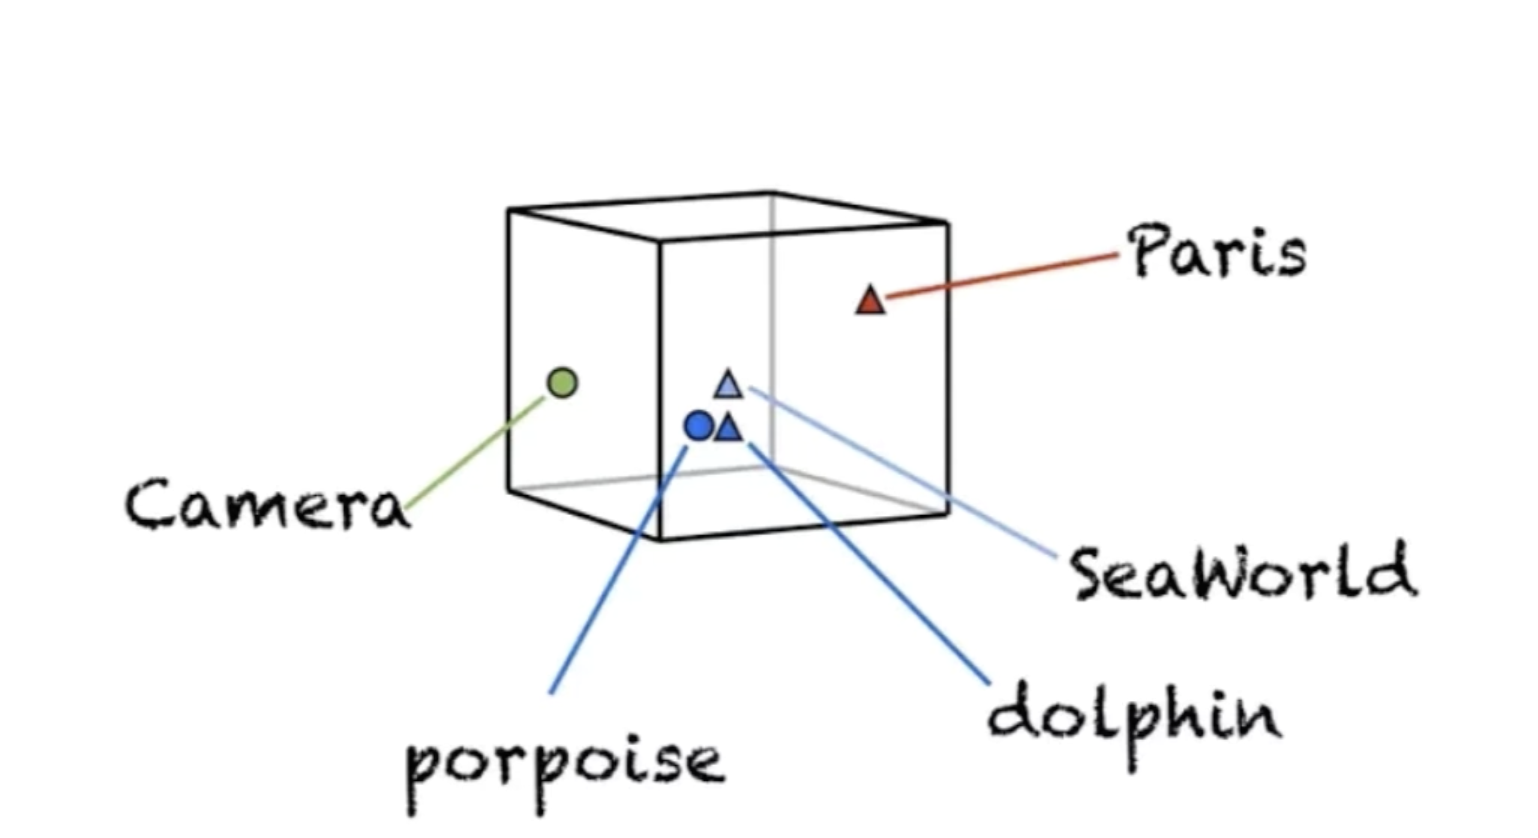
\includegraphics[width=0.8\textwidth]{Figures/word-embeddings}
\end{center}
\end{frame}
%----------------------------------------------------------------------------%

\begin{frame}
\frametitle{Idea}
\begin{itemize}
\item Unsupervised extraction of semantics using large corpus (Wikipedia etc)
\item Input: one-hot representation of word (as in BoW)
\item Use auxiliary task to learn continuous representation
\end{itemize}
\end{frame}
%----------------------------------------------------------------------------%


\begin{frame}
\frametitle{Continious Bow vs SkipGram}
\begin{figure}
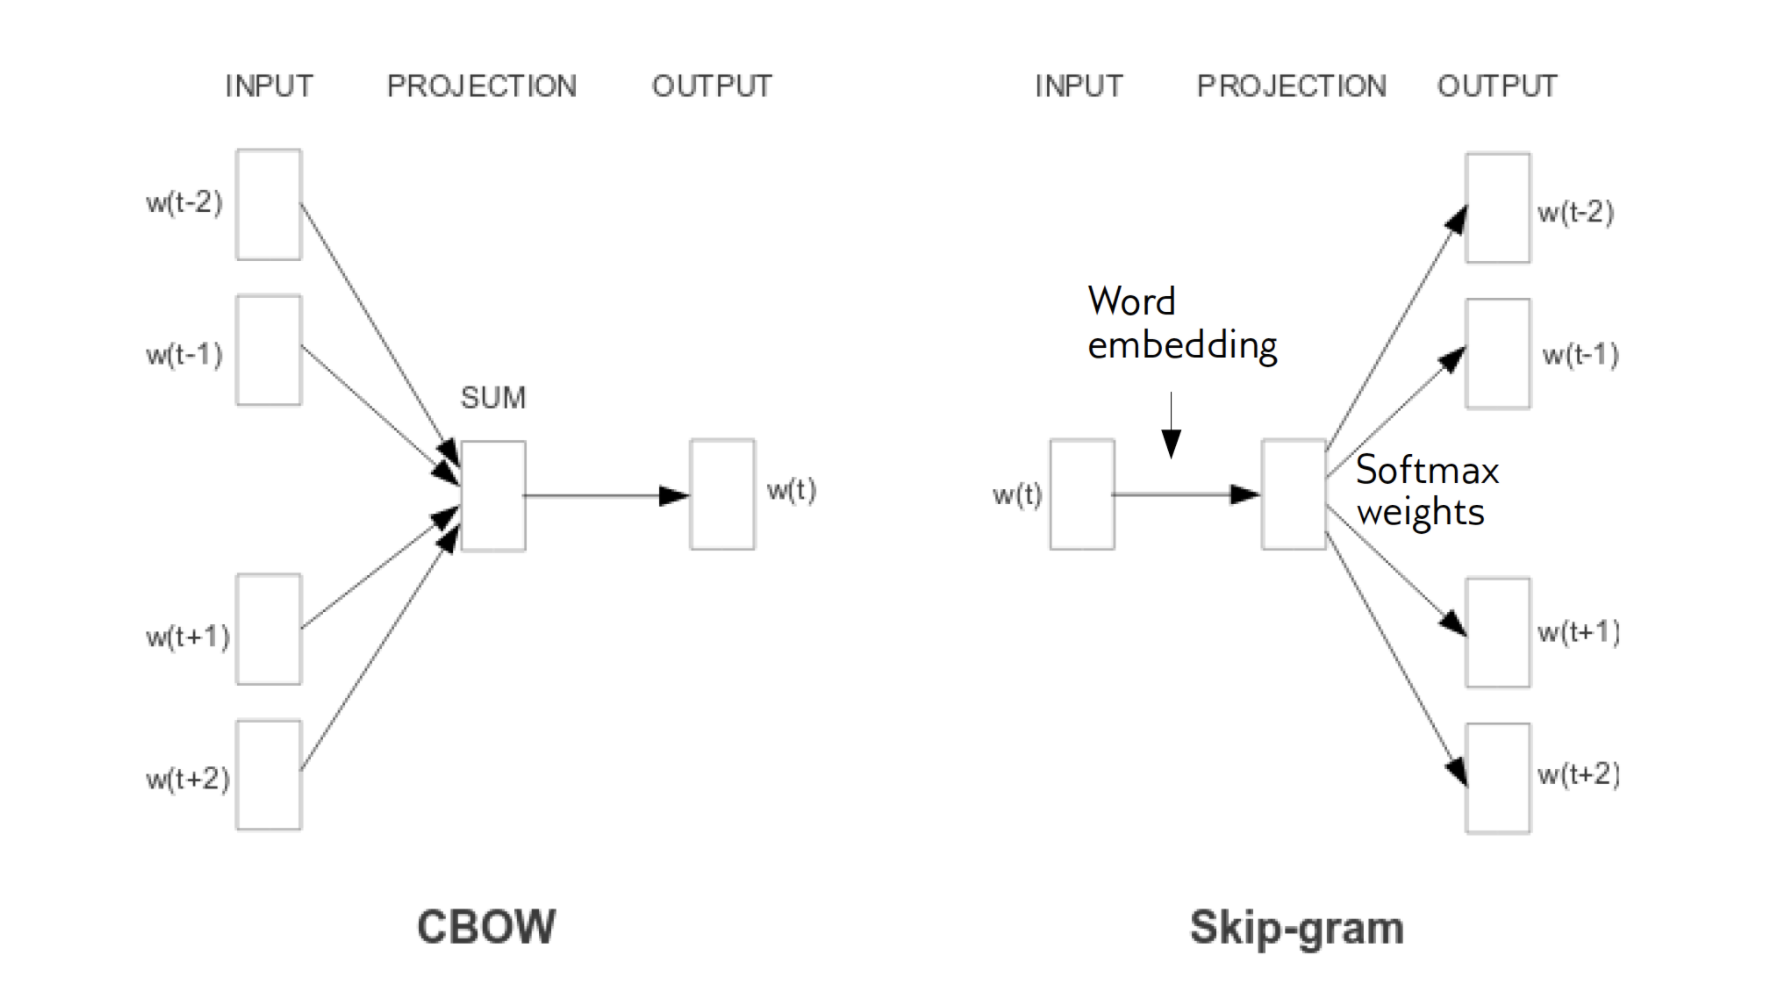
\includegraphics[width=1.1\linewidth ]{Figures/cbow-skipgram}
\end{figure}

\end{frame}


\begin{frame}
\frametitle{Durian Example}

\begin{itemize}
  \item Durian is a tropical fruit known for its sweetness and strong odor
  \item In a word embedding space, similar words tend to have similar vector representations
  \item Let's say we have a word embedding model that maps words to 4-dimensional vectors
  \item The word "durian" might have the following vector representation: \[ \text{{durian}} = \begin{bmatrix} 0.9  \\ -0.4 \\ 0.5 \\  0.6 \end{bmatrix} \]
  \item Other fruits like "mango" and "pineapple" may have similar vector representations
  \item This closeness in the embedding space captures the semantic similarity between these fruits
\end{itemize}

\end{frame}

\begin{frame}
\frametitle{Dense Representation of Words}

\begin{table}[ht]
\centering
\begin{tabular}{|c|c|c|c|c|c|c|}
\hline
\textbf{Dimension} & \textbf{dog} & \textbf{cat} & \textbf{car} & \textbf{house} & \textbf{durian} & \textbf{mango} \\
\hline
\textbf{Dimension 1} & -0.2 & -0.1 & -0.01 & -0.01 & 0.9 & 0.8 \\
\hline
\textbf{Dimension 2} & -0.4 & -0.3 & 0.3 & 0.4 & -0.4 & 0.7 \\
\hline
\textbf{Dimension 3} & 0.9 & 0.9 & -0.02 & -0.01 & 0.5 & 0.5 \\
\hline
\textbf{Dimension 4} &0.6 &  -0.2  & 0.8 & -0.6 & 0.3 & 0.3 \\
\hline
\end{tabular}
\caption{Sample dense representation of words in a 4-dimensional space}
\end{table}

\begin{itemize}
  \item Each word is represented by a dense vector with multiple dimensions (to fix ideas, let't think of Dimension 1 as fruit related, Dimension 2 smell related, Dimension 3 related to living things, and Dimension 4 related to outdoor activities.
  \item Similar words have similar vector patterns across dimensions
  \item Dense representations enable capturing complex relationships between words
\end{itemize}

\end{frame}
%----------------------------------------------------------------------------%
\begin{frame}
\frametitle{Visualizing Analogies}

\begin{center}
    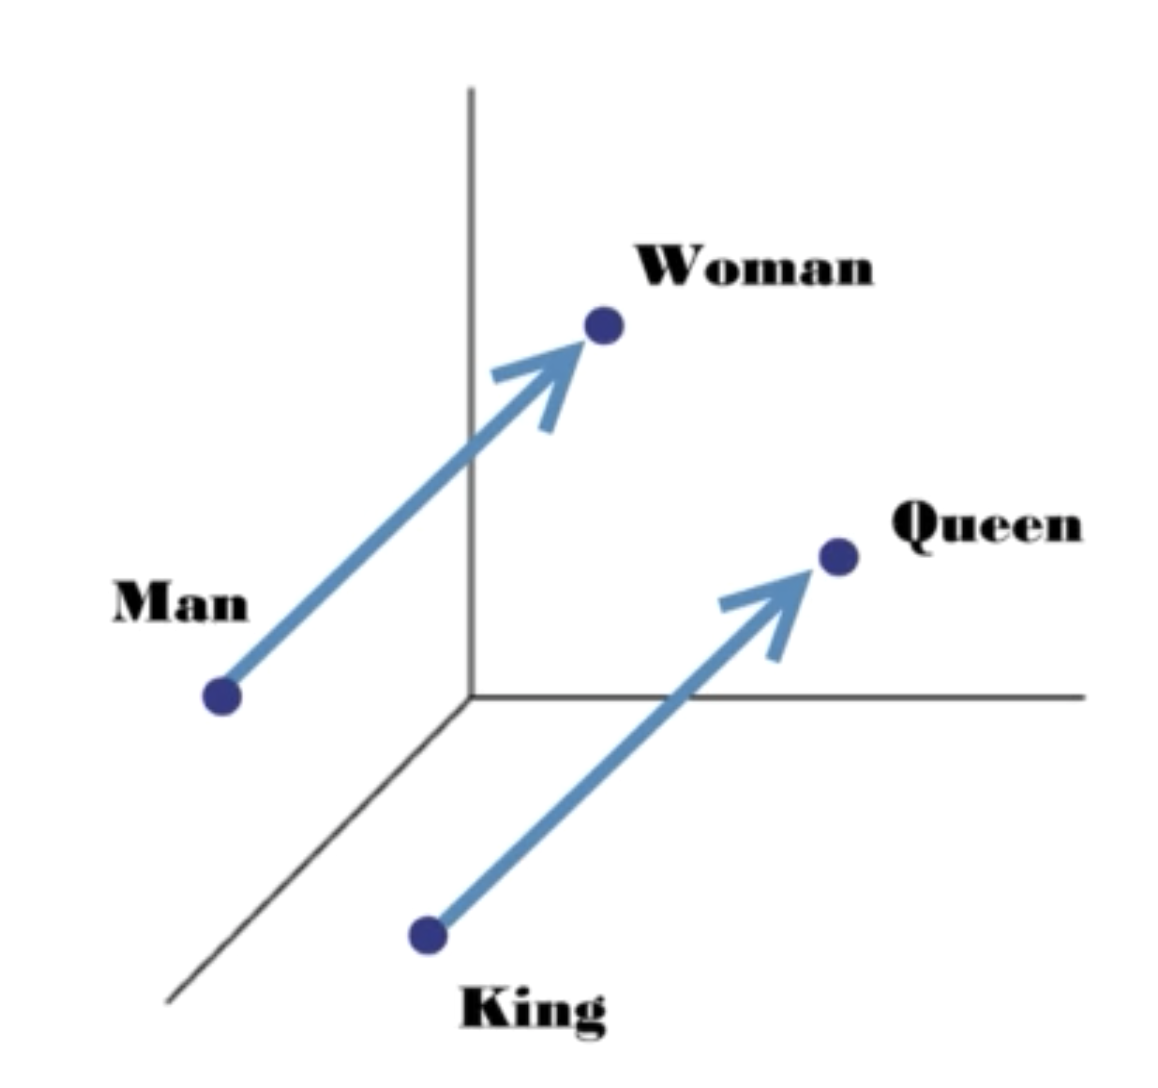
\includegraphics[width=0.7\textwidth]{Figures/visualizing-analogies}
\end{center}
\end{frame}
%----------------------------------------------------------------------------%


%----------------------------------------------------------------------------%
\begin{frame}
\frametitle{Examples}
\begin{itemize}
\item King - Queen $\sim =$ Prince - Princess
\item France - Paris $\sim =$  Germany - Berlin
\item Japan - Japanese $\sim =$  China - Chinese
\item Brother - Sister $\sim = $ Uncle - Aunt
\item Walk - Walking $\sim =$  Swim - Swiming
\end{itemize}

\end{frame}


\end{document}

